\documentclass[a4paper,onecolumn,10pt]{article}
\usepackage[polish]{babel}
\usepackage[utf8]{inputenc}
\usepackage[T1]{fontenc}
\usepackage[left=2.1cm,right=2.1cm]{geometry}
\usepackage[dvipsnames]{xcolor}
\usepackage{amsmath,calc,indentfirst,fancyhdr,amsfonts,graphicx,epstopdf,caption, mathcomp, subcaption,wrapfig, siunitx,pbox,float,algorithm}
\usepackage[noend]{algpseudocode}


\makeatletter
\def\BState{\State\hskip-\ALG@thistlm}
\renewcommand{\ALG@name}{Algorytm}
\makeatother

\renewcommand{\baselinestretch}{1.1}	 % odstep miedzy liniami
\addto\captionspolish{\renewcommand{\figurename}{Wykres}} % zmiana podpisu pod obrazkami, zamiast "Rysunek" bedzie "Wykres"
\newcommand{\NN}{\mathbb{N}}			 % makro do znaku liczb naturalnych

\newcommand{\R}[1]{\textcolor{red}{#1}}  % makro do polecenia z parametrami - tutaj 1 parametr
\newcommand{\G}[1]{\textcolor{green}{#1}} 
\newcommand{\B}[1]{\textcolor{RoyalBlue}{#1}} 
% kolorowanie {\B{argument}}

\newcommand{\PICTURES}{} % szybsza kompilacja dzieki stalej "usuwajacej" obrazki
						 % zakomentowanie \PICTURES powoduje znikniecie obrazkow

\pagestyle{fancy} % formatuj caly dokument
\fancyhead{}
\fancyfoot{}
\renewcommand{\headrulewidth}{0pt}
\fancyfoot[R]{\thepage} % dla stron poza tytulowa nr w prawym dolnym rogu

\fancypagestyle{plain}{ % dla strony tytulowej nr w prawym dolnym rogu
	
	\renewcommand{\headrulewidth}{0pt}
	\fancyhf{}
	\fancyfoot[R]{\thepage}
}

\title{\Large\vspace{-2.5cm}{\Huge S}PRAWOZDANIE - LABORATORIUM NR {\Huge5}\\
		\textbf{Diagonalizacja macierzy metodą potegową} } 
\date{\Large28 marca 2019}
\author{\Large Marek Kiełtyka}

\begin{document}
\maketitle

\vspace{-1.2cm}\section{Wstęp}
	
\subsection{Metoda potęgowa}

Jako jedna z metod iteracyjnych umożliwia numeryczne wyznaczenie pojedynczych wartości i wektorów własnych danej macierzy. Konieczne jest założenie o istnieniu jej $n$ liniowo niezależnych wektorów własnych, które stanowią bazę przestrzeni liniowej postaci $ \vec{x}_1, \vec{x}_2, \dots \vec{x_N} $. Mając do dyspozycji daną bazę, można zdefiniować poniższe równości dla dowolnego wektora $\vec{v}_0$ i pojedynczych wartości własnych $\lambda_i$ macierzy wejściowej.

\begin{alignat*}{3}
\vec{v}_0 &= \sum_{i=1}^N \alpha_i x_i \\
A\vec{v}_0 &= \sum_{i=1}^N \alpha_i \lambda_i x_i \\
\vec{v} &= A^m \vec{v}_0 \implies \vec{v} = \sum_{i=1}^N \alpha_i \lambda_i^m x_i
\end{alignat*}

Jeśli ponadto założy się istnienie słabomalejącego ciągu wartości własnych: 
\begin{equation}
|\lambda_1 | \geq |\lambda_2| \geq \dots \geq |\lambda_N|,
\end{equation}
to można wystosować granicę z $\lambda_1$ jako dominującą wartością własną i na tej podstawie łatwo ją obliczyć.
\begin{equation}
\lim_{m \rightarrow \infty} \frac{A^m \vec{v}_0}{\lambda_1^m} = \alpha_1 x_1 \implies \lambda_1 = \lim_{m \rightarrow \infty} \frac{\vec{y}^T \vec{v}_{m+1}}{\vec{y}^T \vec{v}_m}
\end{equation}
Klasyczna metoda potęgowa umożliwia jednak znalezienie tylko nadmienionej wartości własnej i odpowiadającego jej wektora, toteż na laboratorium wykorzystano pomocniczy algorytm opisany poniżej.
 
\subsection{Pseudokod}

\begin{minipage}{0.5\textwidth}
	\begin{algorithm}[H]
		\centering
		\caption{Iteracyjne wyznaczanie wartości i wektorów własnych metodą potęgową}
		\label{metoda}
		\begin{algorithmic}[1]
		\For{k = 1 to k <= N }
		\State$x^1_k = \left[1,1,\dots,1\right] $
		\For{i = 1 to i <= IT\_MAX }
		\State$x_k^{i+1} = W_k x_k^i$
		\State$\lambda_k^i = \frac{(x_k^{i+1})^T x^i_k}{(x^i_k)^T x^i_k}$ 
		\State$x^i_k = \frac{x^{i+1}_k}{||x^{i+1}_k||_2}$
		\EndFor
		\State$W_{k+1} = W_k - \lambda_kx^i_k(x_k^i)^T $
		\EndFor
		\end{algorithmic}
	\end{algorithm}
\end{minipage}%
\hfill 
\begin{minipage}{0.49\textwidth}
	\begin{itemize}
		\item $ k $ - numer wyznaczanej wartości własnej,
		\item $ i $ - numer iteracji dla określonego $ k $,
		\item $ A $ - macierz pierwotna,
		\item $ W_k $ - macierz iteracji, 
		\item $ \lambda^i_k $ - przybliżenie $ k$-tej wartości własnej w $ i$-tej iteracji,
		\item $ x_i^k $- $ i$-te przybliżenie $ k$-tego wektora własnego,
		\item $ N $ - liczba wartości własnych do wyznaczenia,
		\item \textit{IT\_MAX }$ = 12 $ - maksymalna liczba iteracji dla każdego $ k $.
	\end{itemize}
\end{minipage}
Ciekawostką jest fakt, że podobnego algorytmu używa się w pozycjonowaniu stron internetowych podczas ich\,wyszukiwania.

\section{Zadanie do wykonania}

\subsection{Opis problemu}

Do przetestowania metody użyto macierzy symetrycznej \textit{A} rzędu $N = 7$ danej przepisem
\begin{equation}
a_{i,j} = \frac{1}{\sqrt{2 + |i - j|}} \text{ dla } i,j \in \{1,\dots,7\}.
\end{equation}
Symetryczność macierzy zagwarantowała, że wszystkie wartości własne oraz składowe wektorów własnych były rzeczywiste. Utworzono ponadto macierz iterującą $ W_0 $ będącą wstępnie kopią macierzy $ A $. W celu sprawdzenia poprawności obliczeń zdefiniowano macierz $ D $ z twierdzenia o ortogonalnym podobieństwie, które opisuje wzór
\begin{equation}
D = X^T AX
\label{macierzD}
\end{equation}
gdzie $ X $ to macierz składająca się z kolumn bedących kolejnymi wektorami własnymi macierzy wejściowej:
\begin{equation}
X = 
\begin{bmatrix}
\vec{x}_1, \vec{x}_2, \dots, \vec{x}_N
\end{bmatrix}
.
\end{equation}
Każdy wektor własny $ \vec{x}_k $ był inicjalizowany jedynkami w poszczególnych obiegach pętli. Zgodnie z pseudokodem należało je kolejno przybliżać, wykonując zawsze z góry założoną liczbę iteracji równą \textit{IT\_MAX} $ = 12 $ dla każdej wartości własnej.

\subsection{Wyniki}

Rozwiązanie opracowano w oparciu o bibliotekę\textit{ Numerical Recipes} oraz samodzielnie opracowaną zwaną \textit{ObjectiveNR}, która bazuje na wcześniej wymienionej. Dzięki temu operacje na macierzach i wektorach były intuicyjne i klarowne. Wartości własne zapisano do pliku w celu sporządzenia wykresów ich przybliżeń za pomocą programu \textit{gnuplot}. Co warte podkreślenia, obliczenia zostały wykonane dla liczb pojedynczej precyzji. Poniżej zaprezentowano otrzymane wyniki.

\begin{equation*}
X = 
\begin{pmatrix}
0.352941    &    0.484573   &    -0.475602  &      0.360911    &    0.464092     & -0.0101197   &    -0.262004 \\
0.377935      &  0.171643    &   -0.445369   &    -0.463862     &  -0.223418   &    -0.271684      &  0.519426 \\
0.392221     &  -0.310707     &   -0.26868    &    -0.14009   &    -0.437904    &    0.612246     &  -0.399236 \\
0.396889      & -0.540233    & -0.00402304     &   0.518766    &  -0.0821773     &  -0.506671    &  -0.0014201 \\
0.392221     &  -0.318923     &   0.263991      & -0.140751     &    0.58574      &   0.29737      &  0.401792 \\
0.377935     &   0.157866      &  0.447823      &  -0.46407      &  0.118148      & -0.372767    &   -0.521253 \\
0.352941      &  0.469791       & 0.482709      &   0.36147   &    -0.423249   &     0.259115      &  0.262712
\end{pmatrix}
\end{equation*}

\begin{center}
$ D = $
\end{center}
\begin{equation*}
\begin{pmatrix}
\textbf{3.59586}    &  8.9407e-07  &  -2.98023e-07  &   9.83477e-07  &   -1.2517e-06   & -4.23193e-06  &  -6.19888e-06 \\ 
1.03563e-06   &      \textbf{0.28506}  &   -0.00698455 &   -6.23241e-06 &    3.72529   &          0             &  0 \\ 
-2.90573e-07   &  -0.00698464  &     \textbf{ 0.590373} &   -6.85453e-07 &    1.04308e-07    & 2.23517e-08   & -1.11759e-07 \\
8.90344e-07  &  -6.24917e-06    &-6.59376e-07   &     \textbf{0.122786}   & -0.000102561    & -0.00029791  &  -3.25032e-07 \\
-1.31503e-06  &    2.6077e-08    & 1.04308e-07   & -0.000102531   &     \textbf{0.168944}     & -0.0381233  &  -3.00277e-05  \\
-4.3558e-06  &  -3.72529e-09    & 1.11759e-08     &-0.00029794     & -0.0381233   &    \textbf{0.0942673}   & -5.72642e-05 \\
-6.31623e-06  &  -2.04891e-08   & -1.41561e-07    &-3.21306e-07    & -3.0024e-05   & -5.72731e-05   &   \textbf{ 0.0981543 }
\end{pmatrix}
\end{equation*}
\newpage

\begin{figure}[h!]
	\begin{center}
		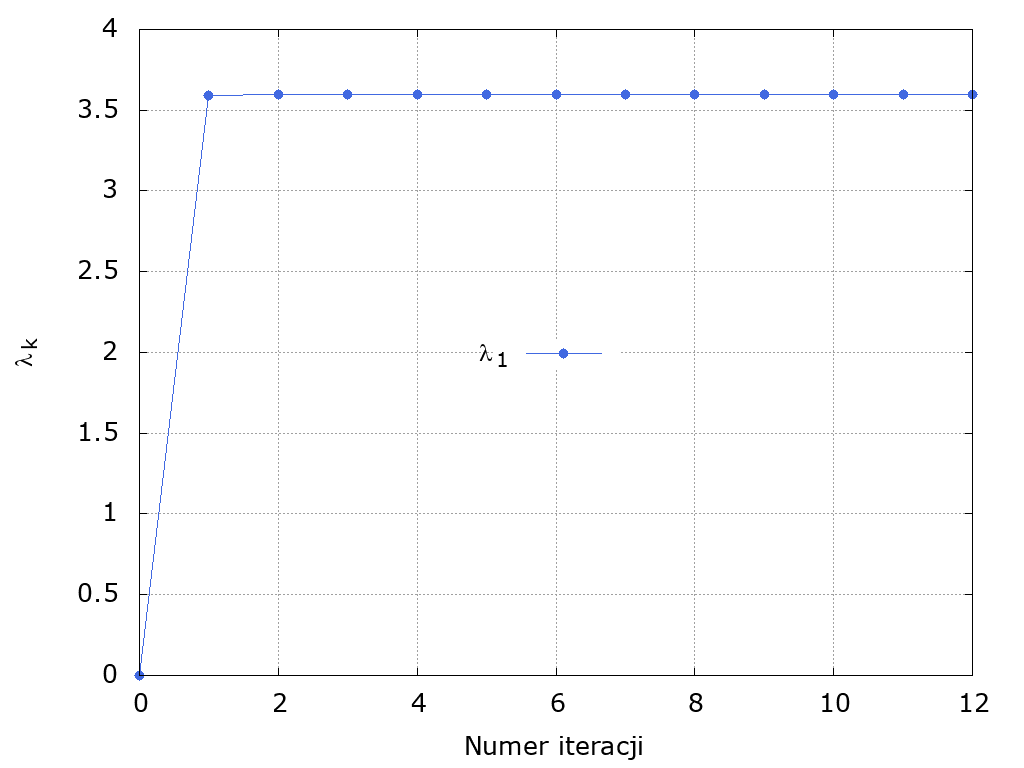
\includegraphics[height=0.43\linewidth]{lambda1.png}
		\caption{Kolejne przybliżenia wartości własnej $ \lambda_1 $ w funkcji numeru iteracji. Wykonano 12 iteracji (bez badania\,zbieżności).}
		\label{lambda1}
	\end{center}
\end{figure}
Dla pozostałych wartości własnych sporządzono wykres (\ref{lambdas}) w celu zachowania czytelności.
\begin{figure}[h!]
	\begin{center}
		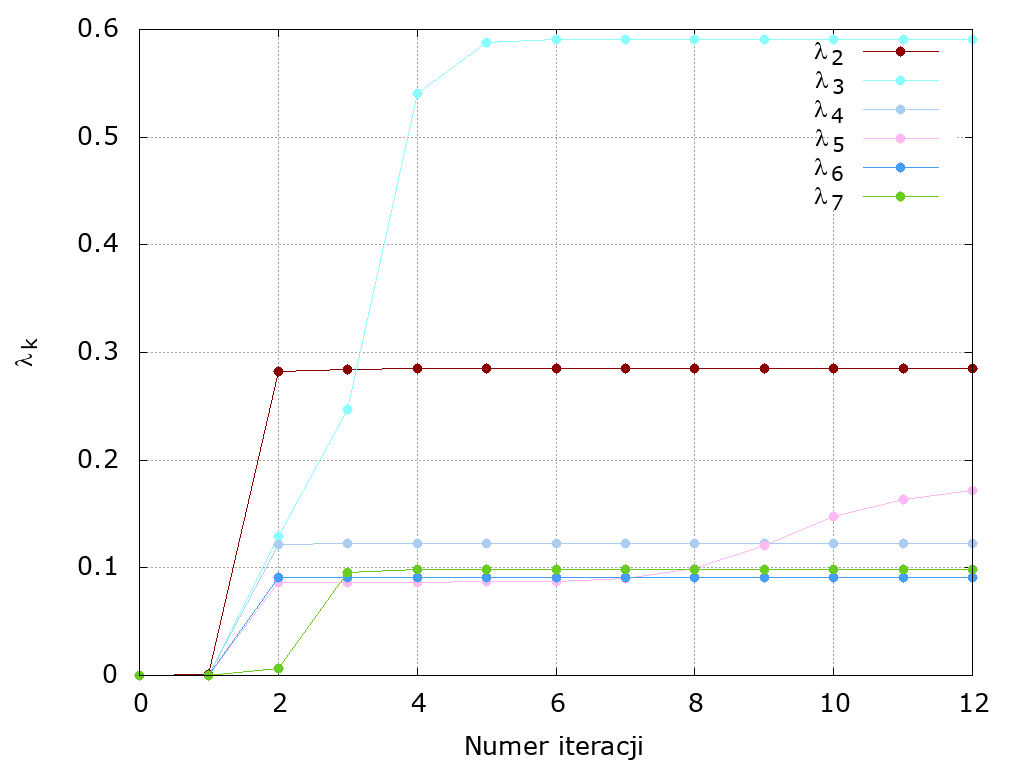
\includegraphics[height=0.43\linewidth]{lambdas.png}
		\caption{Kolejne przybliżenia znalezionych wartości własnych $ \lambda_k $ w funkcji numeru iteracji. Wykonano 12 iteracji (bez badania zbieżności).}
		\label{lambdas}
	\end{center}
\end{figure}

\newpage
\section{Wnioski}
Dowodem na poprawność zaimplementowanej metody jest postać macierzy $D$, która zawiera na diagonali wartości własne odpowiadające kolejnym wektorom własnym przechowywanym w kolumnach macierzy $X$. Pozostałe elementy powinny być w idealnym przypadku równe zeru, lecz przez wgląd na pojedynczą precyzję i niedokładność są tylko zbliżone do niego, jeśli spojrzy się na rząd tych liczb.

Wartości własne nie zostały znalezione w porządku ciągu malejącego. Szeregując je w ten sposób otrzymuje się ciąg
\begin{equation}
|\lambda_1 | \geq |\lambda_3| \geq |\lambda_2|\geq |\lambda_5|\geq |\lambda_4|\geq |\lambda_7| \geq |\lambda_6|.
\end{equation}
Oprócz dominującej wartości, kolejne sąsiednie pojawiły się na wyjściu w odwrotnej kolejności. Ich cechą wspólną jest stosunkowo szybkie osiągnięcie teoretycznej zbieżności, która jednak nie zawsze musi wystąpić (patrząc choćby na $\lambda_5$). Stąd w celu uzyskania bardziej przybliżonych rezultatów powinno się znacząco zwiększyć liczbę iteracji ponad aktualne $12$ powtórzeń.



\end{document}